\documentclass[12pt]{report}
\usepackage{graphicx} % Required for inserting images
\usepackage{natbib}
\usepackage{amsmath}
\usepackage{float}
\usepackage{palatino}
\usepackage{amssymb} 
\usepackage{graphicx}
\usepackage{tabularx}
\graphicspath{ {images/} }
\usepackage[labelfont=bf]{caption}
\usepackage{subcaption}
\usepackage{setspace}
\usepackage{times} %Use times new roman
\captionsetup[table]{font = {stretch=1.35}}
\captionsetup[figure]{font = {stretch=1.35}}
\usepackage[margin=1.3in]{geometry} %1 inch margins
\linespread{1.6} %double spacing
\usepackage[hidelinks]{hyperref}
\usepackage{xcolor}
\usepackage{overpic}
\usepackage{indentfirst}
\usepackage[all]{nowidow}
\usepackage{caption}
\captionsetup{justification=raggedright,singlelinecheck=false}
\usepackage{nccmath}
\usepackage{notoccite}
\usepackage{multirow}
\usepackage{rotating}
\usepackage{longtable}
\usepackage{tikz}
\usepackage{booktabs}


\begin{document}

\chapter*{Previous work Review and Assessment}
With the increasing impact of software applications on today businesses and
activities, software attribute prediction such as effort estimation,
maintainability, defect and quality classification are gaining growing
interest from both academic and industry communities.\\

A research paper by\cite{LARADJI2015388} focuses on the increasing importance
of software attribute prediction, such as effort estimation, maintainability,
defect, and quality classification, due to a growing reliance on software
applications. The paper highlights the limitations of conventional prediction
algorithms such as decision trees, Bayesian methods, and artificial neural
networks multilayer perceptron (ANN-MLP) when handling skewed and redundant
defect datasets. The research introduces ensemble learning's voting mechanism
as a solution, which assigns higher weights to successful individual
classifiers, thereby mitigating the effects of feature irrelevance and
redundancy. The paper's main objective is to demonstrate the positive effect of
feature selection on the performance of defect classification. The findings
suggest that for a dataset with 0.5\% defective components, a classification
accuracy of 99.5\% can be achieved by classifying all components as
non-defective, and an overall accuracy of 99\% can be achieved by a binary
classifier that classifies all data samples as the majority class. In the
discussion section, the paper compares the results of the average probability
ensemble (APE) model with two basic classifiers (W-SVMs and random forests).
The W-SVMs classifier assigns weights inversely proportional to the class
occurrence in the dataset, allowing for potentially better model fitting in the
case of imbalanced datasets. \\

Another paper by\cite{dada2021ensemble} discusses the process of software
defect prediction, which involves identifying likely flawed sections of
software. The paper introduces a model that uses a base layer of Linear
Discriminant Analysis (LDA), K Nearest Neighbors (KNN), and Generalized Linear
Model with Elastic Net Regularization (GLMNet) and a top layer of Random Forest
(RF). The results demonstrate that this model is capable of effectively
handling PROMISE datasets, known for their noisy attributes and high
dimensions. This paper is anticipated to make a significant contribution to the
field of software defect prediction. According to the results, the Ensemble
machine learning technique offers superior prediction accuracy for software
defect prediction, providing a significant insight from this study. The
proposed model achieved an overall prediction accuracy of 88.56\% across all
experimental datasets. Furthermore, the Mean Squared Error (MSE) of the
proposed model is significantly lower than other models, demonstrating that the
Ensemble technique effectively handles errors in the learning model caused by
noise, bias, and variance. Therefore, the research suggests that ensemble
machine learning models provide a robust solution for software defect
prediction.

\chapter*{Methodology}
\section*{Data Collection and Preprocessing}
The NASA Metrics Data Program (MDP) software defect datasets were collected from
various NASA software projects. These datasets encompass information on software
modules each have their own attributes and a binary label indicating whether the
module is defective or not. The datasets were preprocessed to remove any
missing values by imputing the missing values by the mean of the column
and remove duplicates found the datasets.

\section*{Brief Overview of the Task and Models Used}
The task at hand involved a binary classification problem, a common type of
task in the field of machine learning. Binary classification refers to the
process of classifying elements into two distinct groups based on certain
characteristics or features. In this context, the task was to predict whether a
data point belongs to class 0 (majority class) or class 1 (minority class). To
accomplish this task, four different machine learning models were employed.
These models represent a variety of algorithmic approaches and were chosen for
their distinctive strengths in handling classification tasks.

\subsection*{Support Vector Machine}
The Support Vector Machine (SVM) is a widely utilized algorithm in the field of
machine learning, particularly for classification and regression tasks.
According to\cite{Cortes1995}, who first introduced the concept, SVM is a
classifier which performs its task by constructing a hyperplane in a
multi-dimensional space that separates data points of different classes. The
SVM model operates on the principle of maximizing the margin, which is the
distance between the hyperplane (decision boundary) and the nearest data points
from different classes, known as support vectors.

The hyperplane is defined as: \( w \cdot x + b = 0 \) where\dots\\ w is the
weight vector.\\ x is the input data vector.\\ and b is the bias term.\\

The decision function for SVM is given by: \[ f(x)=\mathrm{sign}(w \cdot x + b) \] where\dots \\ $f(x)$ predicts the class label of input vector x.\\
$sign(\cdot)$ returns the sign of its argument.\\

\begin{figure}[ht]
    \centering
    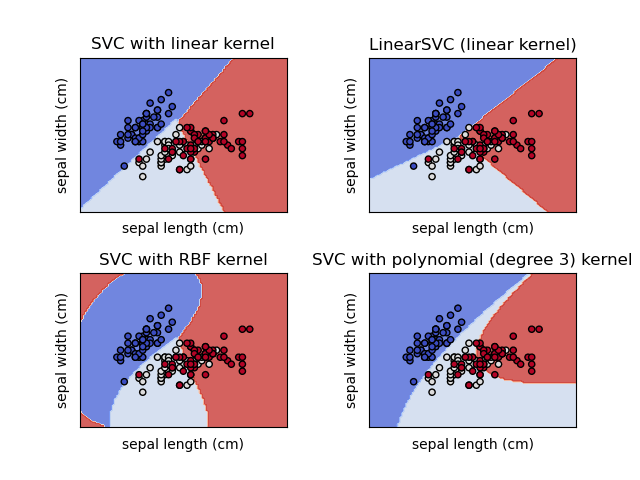
\includegraphics[width=8cm]{./figures/images (4).png}
    \caption{SVM Classifier}\label{fig:fig1}
\end{figure}

In cases where the data is not linearly separable in its original feature
space, SVM can use the kernel trick to implicitly map the data to a
higher-dimensional space where it becomes separable.

\subsubsection{Linear Kernel}
\textbf{Equation}: $K(x_i, x_j) = x_i^T x_j$

\textbf{Explanation}: The linear kernel represents the dot product between the input feature vectors $x_i$ and $x_j$. This kernel is used when the data is linearly separable in the original feature space.

\subsubsection{Polynomial Kernel}
\textbf{Equation}: $K(x_i, x_j) = (\gamma x_i^T x_j + r)^d$

\textbf{Explanation}: The polynomial kernel maps the input data into a higher-dimensional space using a polynomial function. The hyperparameters $d$ and $r$ are user-defined positive integers that control the degree of the polynomial and a constant term, respectively. The parameter $\gamma$ is a scaling factor that influences the dot product.

\subsubsection{Gaussian (RBF) Kernel}
\textbf{Equation}: $K(x_i, x_j) = \exp \left( -\gamma \|x_i - x_j\|^2 \right)$

\textbf{Explanation}: The Radial Basis Function (RBF) kernel measures the similarity between two data points using the Gaussian distribution. It implicitly maps the data into a high-dimensional space, making it suitable for handling nonlinear relationships. The hyperparameter $\gamma$ controls the width of the Gaussian kernel.

\subsubsection{Sigmoid Kernel}
\textbf{Equation}: $K(x_i, x_j) = \tanh(\gamma x_i^T x_j + r)$

\textbf{Explanation}: The sigmoid kernel uses the hyperbolic tangent function to map the data into a higher-dimensional space. This kernel can be useful in some cases, but it is generally less commonly used compared to linear, polynomial, and Gaussian kernels.

\subsubsection{Laplacian Kernel}
\textbf{Equation}: $K(x_i, x_j) = \exp \left( -\frac{\|x_i - x_j\|}{\gamma} \right)$

\textbf{Explanation}: The Laplacian kernel measures the similarity between two
data points using the Laplace distribution. It is similar to the Gaussian kernel
but has a sharper peak, making it robust to outliers.\\

This characteristic makes SVM highly effective in high-dimensional spaces and
in situations where the number of dimensions is greater than the number of
samples\cite{708428}. In addition to performing linear classification, SVMs can
also effectively handle non-linear classification using what is called the
kernel trick, implicitly mapping their inputs into high-dimensional feature
spaces\cite{10.1007/BFb0020217}. In terms of binary classification, the SVM
model seeks a hyperplane that separates the data into two classes while
maximizing the margin between the classes.

\newpage

\subsection*{Random Forest}
Random Forest is a versatile and popular machine learning algorithm known for
its simplicity and diversity. It was first introduced by\cite{Breiman2001} as
an extension of the decision tree algorithm. A Random Forest operates by
constructing a multitude of decision trees at training time and outputting the
class that is the mode of the classes (classification) or mean prediction
(regression) of the individual trees. \\

\begin{figure}[ht]
    \centering
    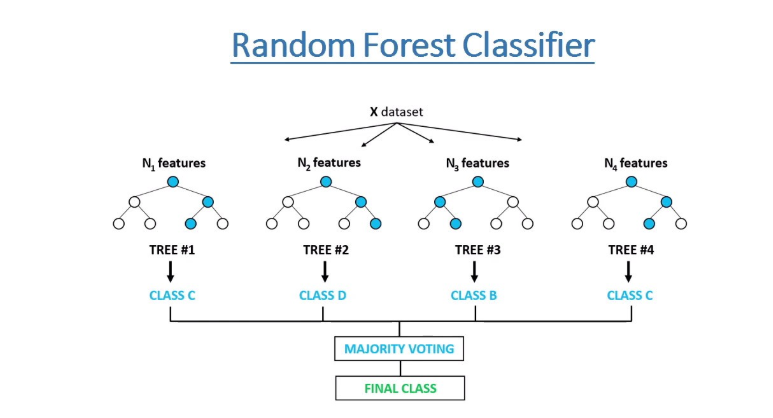
\includegraphics[width=10cm]{./figures/how-random-forest-classifier-work.png}
    \caption{Random Forest}\label{fig:fig2}
\end{figure}

This idea of combining several models to improve the predictive performance is
known as ensemble learning (\cite{Dietterich2000}). Random Forest attempts to
mitigate the high variance problem of individual decision trees, where small
changes in the training set can result in significantly different tree
structures. By averaging the results of a collection of de-correlated trees, it
reduces the risk of overfitting and typically provides a better predictive
performance (\cite{Sagi2018}). Random Forest also has an inherent feature
selection mechanism, as it ranks features (variables) based on their ability to
improve the purity of the node, measured by the Gini impurity or entropy
(\cite{DiazUriarte2006}).

\subsection*{Logistic Regression}
The Logistic Regression model, despite its name, is a powerful tool for binary
classification tasks. This model calculates the probability that a given data
point belongs to a certain class by applying the logistic function to a linear
combination of features\cite{hosmer2013applied}. One of the main advantages of
Logistic Regression is its interpretability. Each feature is assigned a
coefficient that describes its relative importance and direction of association
with the assumes that there is a linear relationship between the log-odds of
the dependent variable and the independent variables. It also requires that the
observations be independent, and the absence of multicollinearity among the
independent variables\cite{peng2002introduction}. The equation of logistic
function or logistic curve is a common “S” shaped curve defined by the below
equation. The logistic curve is also known as the sigmoid
curve\cite{sharma2022logistic}. the formula of logistic function: \[ P=\frac{1}{1+e^{-\left(\beta_0+\beta_1 x\right)}} \]
where..\\$$ {-\left(\beta_0+\beta_1 x\right)} $$ is linear function

\begin{figure}[ht]
    \centering
    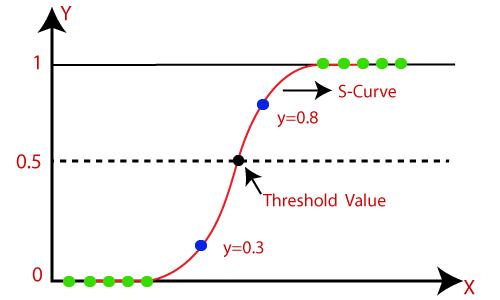
\includegraphics[width=6cm]{./figures/logistic-regression-in-machine-learning.png}
    \caption{Logistic function}\label{fig:fig3}
\end{figure}

\newpage
\subsection*{Ensemble Model}
Ensemble Models are powerful machine learning tools that combine multiple base
models to improve prediction accuracy and robustness over a single model. The
central idea behind ensemble models, often referred to as the ``Wisdom of the
Crowd'', is that a group of weak learners can come together to form a strong
learner\cite{dietterich2000ensemble}.\newline

There are several types of ensemble methods, including Bagging, Boosting, and
Stacking. Bagging, or Bootstrap Aggregating, involves training each model in
the ensemble using a randomly drawn subset of the training set. Boosting is a
sequential process, where each subsequent model attempts to correct the
mistakes of the previous models. Stacking involves training a model to combine
the predictions of several other models\cite{wolpert1992stacked}. Ensemble
models have been shown to significantly increase accuracy on a variety of
tasks, including both regression and classification problems\cite{opitz1999popular}.\newpage
\begin{figure}[ht]
    \centering
    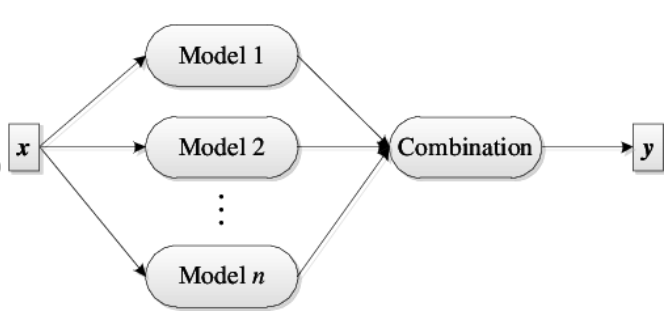
\includegraphics[width=10cm]{./figures/vottingpic.png}
    \caption{Ensemble Model}\label{fig:fig4}
\end{figure}

They tend to be more robust to noise, outliers, and overfitting, as they
average out biases, reduce variance, and are not likely to model random noise
in the output data\cite{zhou2012ensemble}. However, ensemble models can be
computationally expensive and may require more time to train and predict than
individual models. Also, they may suffer from complexity, which may make them
harder to interpret than individual models\cite{rokach2010ensemble}.\newpage

\subsection*{Performance Metrics}
In machine learning, the performance of a model is evaluated based on certain
metrics that depend on the nature of the task whether it is a classification,
regression, or clustering task. This paper focuses on the metrics used to
evaluate classification models, including accuracy, precision, recall,
F1-score, and Area Under the Receiver Operating Characteristic curve (AUROC).
Accuracy, the ratio of correctly predicted observations to the total
observations, is the most straightforward measure but can be misleading in case
of imbalanced classes\cite{powers2011evaluation}.\[ \text { Accuracy }=\frac{(T P+T N)}{(T P+T N+F P+F N)} \] Precision, the ratio of correctly
predicted positive observations to the total predicted positives, is an
essential metric when the cost of false positives is high\cite{sokolova2009systematic}.\[ \text { Precision }=\frac{T P}{(T P+F P)} \]
Recall measures the ratio of correctly predicted positive observations to all
observations in the actual class, and is crucial when the cost of false
negatives is high\cite{sokolova2009systematic}.\[ \text { Recall }=\frac{T P}{(T P+F N)} \] The F1-score is the weighted average of precision and recall
and is typically more useful than accuracy, particularly for uneven class
distributions\cite{van1979information}. \[ F 1 \text { Score }=\frac{2 T P}{(2T P+F P+F N N)} \]

% \subsubsection{Cross validation}
% According to\cite{kohavi1995}, Cross-validation is a powerful preventative
% measure against overfitting. The technique is used to assess how the results of
% a statistical analysis will generalize to an independent data set. It is a
% popular method because it is simple to understand and because it generally
% results in a less biased or less optimistic estimate of the model skill than
% other methods, such as a simple train/test split. In machine learning, we
% cannot fit the model on the training data and say the model will work well with
% the real-world data. We need some kind of assurance or approximation about how
% our model will behave in the future or unseen data. This is where
% Cross-validation plays a crucial role.\\

% ~\cite{kohavi1995} explained that Cross-validation is a resampling procedure used to evaluate machine learning models on a limited data sample. It provides a more accurate method of measuring the performance of a model, which helps in improving the model's performance and optimizing the hyperparameters. The most common type of cross-validation, and the one often referred to by this name, is k-fold cross-validation. In k-fold cross-validation, you divide your data points into k subsets of roughly equal size. You then run k separate learning experiments:

% \begin{itemize}
%     \item Randomly partition the data into k equal sized subsets. One of the k subsets is
%           used as the test set, and the other k-1 subsets are put together to form a
%           training set.
%     \item Train a machine learning model on the k-1 training sets and test the model on
%           the test set, recording the test set error rate.
%     \item  Repeat the process k times, each time using a different subset as your test
%           set.
% \end{itemize}

% Finally, compute the average of the k test set error rates. This is the
% cross-validation error rate, an estimate of the model's prediction error. This
% process is illustrated in the figure below:

% \begin{figure}[hbt!]
%     \centering
%     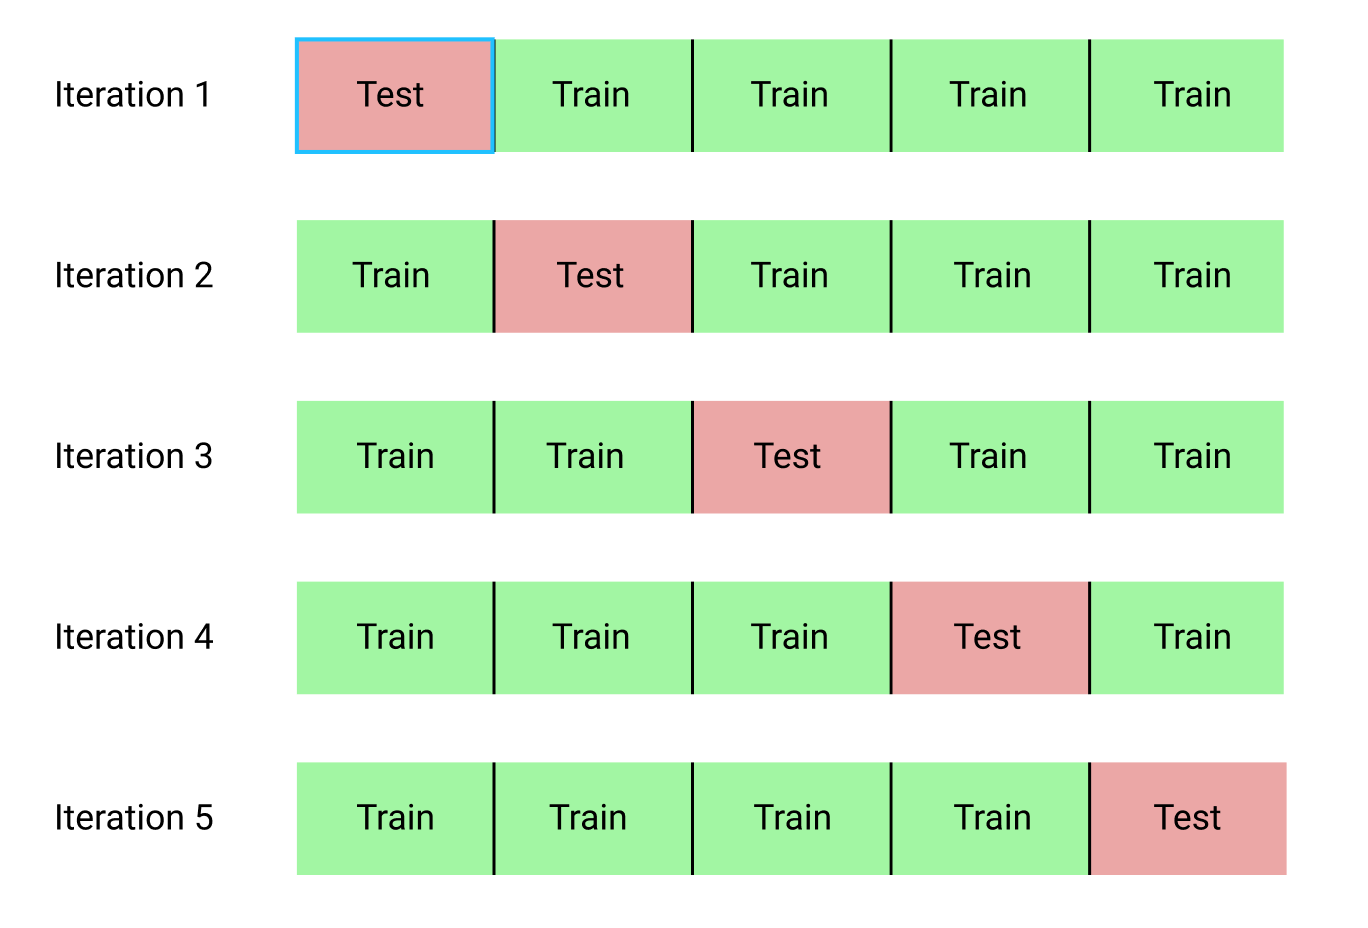
\includegraphics[width=0.8\textwidth]{./figures/kfold.png}
%     \caption{kfold}\label{fig:kfold}
% \end{figure}

\section*{Model performance analysis}
Four different machine learning models were evaluated in this study, which
included Support Vector Machine (SVM), Random Forest, Logistic Regression, and
an Ensemble model. The performance of these models was assessed based on a
binary classification task.\\

% Accuracy
\begin{table}[hbt!]
      \centering
      \caption{Accuracies for each model on all datasets}
      \label{tab:model-performance2}
      \resizebox{\textwidth}{!}{%
            \begin{tabular}{lrrrrrrrrrrrrr}
                  \toprule
                  Model               & CM1 & JM1 & KC1 & KC3 & KC4 & MC1 & MC2 & MW1 & PC1 & PC2 & PC3 & PC4 & PC5 \\
                  \midrule
                  SVM                 & 0.9 & 0.8 & 0.8 & 0.8 & 0.7 & 1.0 & 0.7 & 0.8 & 0.9 & 1.0 & 0.9 & 0.9 & 0.8 \\
                  Random Forest       & 0.8 & 0.8 & 0.7 & 0.9 & 0.8 & 0.9 & 0.8 & 0.8 & 0.9 & 1.0 & 0.9 & 0.9 & 0.8 \\
                  Logistic Regression & 0.8 & 0.8 & 0.7 & 0.8 & 0.7 & 1.0 & 0.7 & 0.9 & 0.9 & 1.0 & 0.9 & 0.9 & 0.8 \\
                  Voting Classifier   & 0.9 & 0.8 & 0.7 & 0.8 & 0.7 & 1.0 & 0.7 & 0.9 & 0.9 & 1.0 & 0.9 & 0.9 & 0.8 \\
                  \bottomrule
            \end{tabular}
      }
\end{table}

% Table for recall
\begin{table}[hbt!]
      \centering
      \caption{Recall for each model on all datasets}
      \label{tab:model-performance}
      \resizebox{\textwidth}{!}{%
            \begin{tabular}{lrrrrrrrrrrrrr}
                  \toprule
                  Model               & CM1 & JM1 & KC1 & KC3 & KC4 & MC1 & MC2 & MW1 & PC1 & PC2 & PC3 & PC4 & PC5 \\
                  \midrule
                  SVM                 & 0.0 & 0.0 & 0.1 & 0.1 & 0.6 & 0.0 & 0.6 & 0.1 & 0.2 & 0.0 & 0.0 & 0.4 & 0.2 \\
                  Random Forest       & 0.0 & 0.2 & 0.3 & 0.0 & 0.9 & 0.0 & 0.4 & 0.0 & 0.1 & 0.0 & 0.1 & 0.4 & 0.4 \\
                  Logistic Regression & 0.0 & 0.1 & 0.2 & 0.1 & 0.6 & 0.1 & 0.6 & 0.3 & 0.3 & 0.0 & 0.3 & 0.5 & 0.3 \\
                  Voting Classifier   & 0.0 & 0.1 & 0.2 & 0.1 & 0.6 & 0.0 & 0.6 & 0.1 & 0.2 & 0.0 & 0.0 & 0.4 & 0.3 \\
                  \bottomrule
            \end{tabular}
      }
\end{table}

% Table for precision
\begin{table}[hbt!]
      \centering
      \caption{Precision for each model on all datasets}
      \label{tab:model-performance}
      \resizebox{\textwidth}{!}{%
            \begin{tabular}{lrrrrrrrrrrrrr}
                  \toprule
                  Model               & CM1 & JM1 & KC1 & KC3 & KC4 & MC1 & MC2 & MW1 & PC1 & PC2 & PC3 & PC4 & PC5 \\
                  \midrule
                  SVM                 & 0.0 & 0.7 & 0.8 & 0.2 & 0.7 & 0.0 & 0.6 & 0.5 & 0.7 & 0.0 & 0.0 & 0.9 & 0.9 \\
                  Random Forest       & 0.0 & 0.5 & 0.6 & 0.0 & 0.8 & 0.0 & 1.0 & 0.0 & 0.5 & 0.0 & 0.3 & 0.9 & 0.6 \\
                  Logistic Regression & 0.0 & 0.6 & 0.5 & 0.2 & 0.8 & 0.5 & 0.6 & 0.8 & 0.5 & 0.0 & 0.5 & 0.9 & 0.7 \\
                  Voting Classifier   & 0.0 & 0.6 & 0.6 & 0.3 & 0.7 & 0.0 & 0.7 & 1.0 & 0.7 & 0.0 & 0.5 & 0.9 & 0.8 \\
                  \bottomrule
            \end{tabular}
      }
\end{table}
% Table for f1-score
\begin{table}[hbt!]
      \centering
      \caption{F1-scores for each model on all datasets}
      \label{tab:model-performance}
      \resizebox{\textwidth}{!}{%
            \begin{tabular}{lrrrrrrrrrrrrr}
                  \toprule
                  Model               & CM1 & JM1 & KC1 & KC3 & KC4 & MC1 & MC2 & MW1 & PC1 & PC2 & PC3 & PC4 & PC5 \\
                  \midrule
                  SVM                 & 0.0 & 0.1 & 0.2 & 0.2 & 0.7 & 0.0 & 0.6 & 0.1 & 0.3 & 0.0 & 0.0 & 0.5 & 0.3 \\
                  Random Forest       & 0.0 & 0.3 & 0.4 & 0.0 & 0.8 & 0.0 & 0.6 & 0.0 & 0.2 & 0.0 & 0.1 & 0.5 & 0.5 \\
                  Logistic Regression & 0.0 & 0.2 & 0.3 & 0.2 & 0.7 & 0.2 & 0.6 & 0.5 & 0.4 & 0.0 & 0.4 & 0.6 & 0.4 \\
                  Voting Classifier   & 0.0 & 0.1 & 0.3 & 0.2 & 0.7 & 0.0 & 0.7 & 0.2 & 0.3 & 0.0 & 0.1 & 0.5 & 0.4 \\
                  \bottomrule
            \end{tabular}
      }
\end{table}
In conclusion, although high accuracy was demonstrated by all models, But the
other metrics were low. These results indicated the presence of class imbalance
in the dataset, a common problem in machine learning tasks. Despite high
accuracy was demonstrated by all models, difficulties were encountered in
effectively classifying the minority class (True). Strategies such as
resampling techniques suggested to address this issue. The model's performance
should not only be assessed on overall accuracy but also on its ability to
identify each class accurately, especially when dealing with imbalanced
datasets.

Feature selection is a crucial step in the machine learning pipeline. It is the
process of selecting the most relevant features from the original dataset to
use in model training. The aim is to enhance the performance of the machine
learning model By using feature selection, we can simplify data entry, reduce
size, and improve model performance in several ways according to\cite{guyon2003introduction}:

\begin{itemize}
    \item Reduce overfitting: Feature selection helps prevent overfitting by focusing on
          the most important features that contain the most predictive information.
    \item Faster training: Reducing the number of features shortens the training time of
          a machine learning as there is less data to process in the model.
    \item Enhanced interpretation: We can improve the interpretation of models by
          selecting the most important features. This means we can better understand
          which features are relevant to the model's predictions and extract insights
          from the model's behavior.

\end{itemize}

According to\cite{kohavi1997}, The wrapper method is a type of feature
selection technique that relies on the performance of a machine learning model
to evaluate the importance of features. It involves training a model on a
subset of features, evaluating its performance, and using that information to
decide whether to add or remove features. This process repeats until it reaches
an optimal set of features. The wrapper method is computationally expensive as
it involves evaluating the performance of a machine learning model for every
possible combination of features. However, it often provides a better
performing feature set compared to other methods, like filter methods, because
it takes into account the interaction of features. There are different types of
wrapper methods, including forward selection, backward elimination, and
recursive feature elimination. Forward selection starts with an empty set and
adds one feature at a time. Backward elimination starts with all features and
removes one feature at a time. Recursive feature elimination is a greedy
optimization algorithm that aims to find the best performing feature subset.\\

\subsubsection*{Recursive Feature Elimination with Cross-Validation (RFECV)}
\subsubsection*{Chi-Squared Feature Selection}
RFECV (Recursive Feature Elimination with Cross-Validation) is a powerful
technique for feature selection in machine learning that fits a model and
removes the weakest feature (or features) until the specified number of
features is reached as mentioned by\cite{guyon2002}. Features are ranked and
by recursively eliminating a small number of features per loop, RFECV attempts
to eliminate dependencies and collinearity that may exist in the model. It
combines the strengths of recursive feature elimination (RFE) and
cross-validation to provide a robust and efficient method for selecting the
most important features and optimizing the performance of a machine learning
model.\\

RFECV then selects the optimal number of features based on the cross-validation
score. The cross-validation score generally increases with the number of
features. However, the score may also increase due to overfitting. RFECV solves
this problem by selecting the number of features for which the cross-validation
score is maximum. RFECV works by iteratively eliminating the least important
features in a dataset, while using cross-validation to evaluate the performance
of the model. The process can be broken down into the following steps:

\begin{itemize}
    \item Initialize the model with all the features: The first step is to initialize the
          model with all the features in the dataset.
    \item Perform cross-validation: The next step is to perform cross-validation on the
          dataset, using the initialized model. This involves splitting the dataset into
          training and testing sets, and evaluating the model's performance on the
          testing sets.
    \item Eliminate the least important features: Based on the performance of the model
          in the cross-validation step, the least important features are eliminated from
          the dataset.
    \item Repeat steps 2--3: Steps 2--3 are repeated until a stopping criterion is met,
          such as a maximum number of iterations or a minimum number of features.
    \item Evaluate the final model: The final model is evaluated on the entire dataset to
          determine its performance.
\end{itemize}

according to\cite{10.3389/fbioe.2020.00496}, RFECV has several advantages over
other feature selection. RFECV can improve the accuracy of a machine learning
model by selecting the most important features. It is computationally
efficient, as it only requires a single pass through the dataset to eliminate
the least important features. Also, provides interpretable results, as it
eliminates features one at a time, allowing for feature importance to be easily
understood. However, RFECV needs a specified or calculable measure of
importance provided by the estimator to perform its operations. Therefore, it
doesn't work with all kinds of models. For instance, it won't work directly
with models like KNN, SVM with non-linear kernel as these models do not provide
a straightforward measure of feature importance.\newpage

% \subsection*{Hyperparameter Tuning}
% Hyperparameter tuning is a fundamental step in the construction of machine
% learning models. The performance of many machine learning algorithms depends on
% their hyperparameters. These are the configuration variables that govern the
% training process itself. This process involves adjusting the parameters of a
% model to improve its accuracy and performance. The optimal hyperparameters for
% a model can significantly differ based on the data and problem at hand,
% necessitating a comprehensive search for the most suitable values. For example,
% the learning rate for training a neural network, the C and sigma in a support
% vector machine. They are not learned by the model during training and must be
% set prior to training. Manual tuning of these hyperparameters is often tedious
% and suboptimal, leading to inefficient use of computational resources. Grid
% search is often the go-to method for hyperparameter tuning, but it suffers from
% the curse of dimensionality. The number of hyperparameter combinations to be
% searched grows exponentially with the number of hyperparameters, making grid
% search computationally very expensive.\\

% \subsubsection*{Random search technique}
% Random search is a technique where random combinations of the hyperparameters are used to
% find the best solution for the built model. It is one of the most commonly used methods
% for hyperparameter optimization.The method was first proposed by\cite{bergstra2012random}.
% Random search contrasts with grid search in that it does not exhaustively try all the parameter
% combinations, but rather samples a fixed number of parameter sets at random from the parameter space.

% The procedure of random search can be summarized as follows:
% \begin{itemize}
%     \item Define a domain of possible values for each hyperparameter.
%     \item Define a budget of the total number of hyperparameter configurations to try.
%     \item For each iteration within the budget, sample a configuration of hyperparameters
%           from the defined domain at random.
%     \item Train a model with the selected hyperparameter configuration and evaluate it.
%     \item Select the hyperparameter configuration that yields the best performance on the
%           validation set.
% \end{itemize}

% The main advantage of random search is its simplicity and efficiency. It is
% straightforward to implement and computationally much more efficient than
% exhaustive search methods like grid search. Furthermore, according to Bergstra
% and Bengio's research, random search is more efficient for hyperparameter
% optimization than grid search when considering the same computational budget.
% However, a potential disadvantage of random search is that it might not find
% the optimal hyperparameters if the budget is not big enough, especially if the
% hyperparameter space is large. It is also possible that random search spends
% too much time exploring irrelevant regions of the hyperparameter space.\newpage

\section*{Model performance analysis}
Four different machine learning models were evaluated in this study, which
included Support Vector Machine (SVM), Random Forest, Logistic Regression, and
an Ensemble model. The performance of these models was assessed based on a
binary classification task.\\

\subsection*{PC1 Dataset Model Performance Analysis}
An accuracy of 92\% was achieved by the SVM model. However, the model's
performance was found to be poor when classifying the minority class (1), with
precision, recall, and f1-score all recorded at 0.00. On the other hand, the
majority class (0) was well-classified by the model with a precision of 0.93,
recall of 0.99, and f1-score of 0.96. The Random Forest model reported an
overall accuracy of 91\%. A relatively poor performance was observed for the
minority class (1) with a precision of 0.20, recall of 0.07, and f1-score of
0.11. The majority class (0) was well-classified with a precision of 0.93, a
recall of 0.98, and an f1-score of 0.95. The Logistic Regression model showed
an overall accuracy of 90\%. It was noted that the model failed to classify any
instance of the minority class (1) correctly, resulting in a precision, recall,
and f1-score all at 0.00. A good performance was observed for the majority
class (0) with a precision of 0.92, a recall of 0.97, and an f1-score of 0.95.
The Ensemble model, with an overall accuracy of 91\%, also failed to correctly
classify any instance of the minority class (1), resulting in precision,
recall, and f1-score of 0.00. A good performance was observed for the majority
class (0) with a precision of 0.93, a recall of 0.98, and an f1-score of
0.95.\\

\begin{table}[ht]
    \centering
    \begin{tabular}{|c|c|c|c|c|}
        \hline
        Model               & Class   & Precision & Recall & F1-score \\
        \hline
        SVM                 & Class 0 & 0.93      & 0.99   & 0.96     \\
        SVM                 & Class 1 & 0.00      & 0.00   & 0.00     \\
        \hline
        Random Forest       & Class 0 & 0.93      & 0.98   & 0.95     \\
        Random Forest       & Class 1 & 0.20      & 0.07   & 0.11     \\
        \hline
        Logistic Regression & Class 0 & 0.92      & 0.97   & 0.95     \\
        Logistic Regression & Class 1 & 0.00      & 0.00   & 0.00     \\
        \hline
        Ensemble Model      & Class 0 & 0.93      & 0.98   & 0.95     \\
        Ensemble Model      & Class 1 & 0.00      & 0.00   & 0.00     \\
        \hline
    \end{tabular}
    \caption{PC1 Dataset Model Performance Analysis.}
    \label{tab:PC1 Performance Analysis}
\end{table}
% \subsection*{\centering Support Vector Machine (SVM)}

% \begin{center}
% \begin{tabular}{|c|c|c|c|}
% \hline
%  & Precision & Recall & F1-score \\
% \hline
% Class 0 & 0.93 & 0.99 & 0.96 \\
% Class 1 & 0.00 & 0.00 & 0.00 \\
% \hline
% \end{tabular}
% \end{center}\\

% The SVM model achieved an accuracy of 92\%. However, its performance when classifying the minority class (1) was poor, with precision, recall, and F1-score all recorded at 0.00. \\

% \subsection*{\centering Random Forest}

% \begin{center}
% \begin{tabular}{|c|c|c|c|}
% \hline
%  & Precision & Recall & F1-score \\
% \hline
% Class 0 & 0.93 & 0.98 & 0.95 \\
% Class 1 & 0.20 & 0.07 & 0.11 \\
% \hline
% \end{tabular}
% \end{center}\\

% The Random Forest model reported an overall accuracy of 91\%. A relatively poor performance was observed for the minority class (1) with a precision of 0.20, recall of 0.07, and F1-score of 0.11. \\

% \subsection*{\centering Logistic Regression}

% \begin{center}
% \begin{tabular}{|c|c|c|c|}
% \hline
%  & Precision & Recall & F1-score \\
% \hline
% Class 0 & 0.92 & 0.97 & 0.95 \\
% Class 1 & 0.00 & 0.00 & 0.00 \\
% \hline
% \end{tabular}
% \end{center}\\

% The Logistic Regression model showed an overall accuracy of 90\%. It failed to classify any instance of the minority class (1) correctly, resulting in a precision, recall, and F1-score all at 0.00. \\

% \subsection*{\centering Ensemble Model}

% \begin{center}
% \begin{tabular}{|c|c|c|c|}
% \hline
%  & Precision & Recall & F1-score \\
% \hline
% Class 0 & 0.93 & 0.98 & 0.95 \\
% Class 1 & 0.00 & 0.00 & 0.00 \\
% \hline
% \end{tabular}
% \end{center}\\

% The Ensemble model has an overall accuracy of 91\%. However, it also failed to classify any instance of the minority class (1) correctly, resulting in precision, recall, and f1-score of 0.00. Its performance on the majority class (0) was good with a precision of 0.93, recall of 0.98, and f1-score of 0.95.\\

\newpage
In conclusion, although high accuracy was demonstrated by all models, difficulties were encountered in effectively classifying the minority class (1). These results indicated the presence of class imbalance in the dataset, a common problem in machine learning tasks. Despite high accuracy was demonstrated by all models, difficulties were encountered in effectively classifying the minority class (1). Strategies such as resampling techniques suggested to address this issue. The model's performance should not only be assessed on overall accuracy but also on its ability to identify each class accurately, especially when dealing with imbalanced datasets.

\chapter*{Proposed Enhancement to Defect prediction Model}

\section*{The Problem with Imbalanced Data Sets}
Class imbalance is a common problem in machine learning classification where there are a disproportionate ratio of observations in each class. Class imbalance can be found in many different areas including medical diagnosis, spam filtering, and fraud detection. The main issue with class imbalance is that most machine learning algorithms work best when the number of samples in each class are about equal. This is because most algorithms are designed to maximize accuracy and reduce error.

\section*{Synthetic Minority Over-sampling Technique (SMOTE)}

Synthetic Minority Over-sampling Technique, or SMOTE, is a popular algorithm to
create synthetic observations of the minority class. It was presented by
\cite{chawla2002smote}.\\

\newpage
SMOTE works by selecting examples that are close in the feature space, drawing a line between the examples in the feature space and drawing a new sample at a point along that line. Specifically, a random example from the minority class is first chosen. Then k of the nearest neighbors for that example are found (typically k=5). A randomly selected neighbor is chosen and a synthetic example is created at a randomly selected point between the two examples in feature space.

\begin{figure}[hbt!]
    \centering
    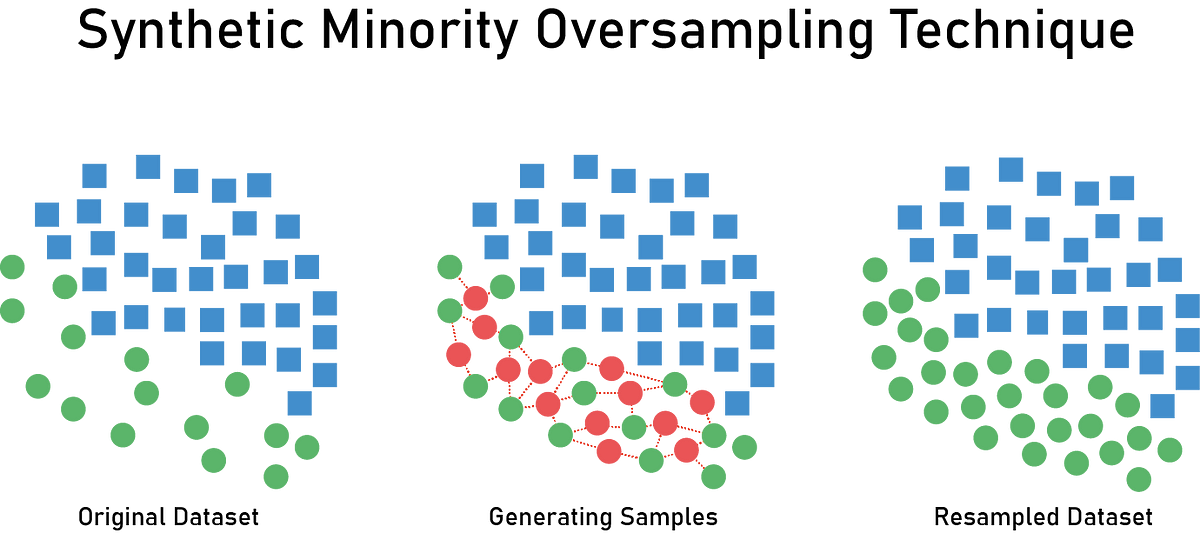
\includegraphics[width=0.9\textwidth]{./figures/smote.png}
    \caption{SMOTE}
    \label{fig:SMOTE}
\end{figure}

The algorithm can be summarized as follows:
\begin{itemize}
    \item For each sample in the minority class, calculate the k nearest neighbors.
    \item From the k neighbors, a neighbor is randomly selected.
    \item A synthetic sample is created by choosing a point between the two instances in
          feature space.
\end{itemize}

This process is repeated until the data is balanced.

\subsection*{Efficacy and Limitations of SMOTE}

According to \cite{fernandez2018smote}, the main advantage of SMOTE is that it
can improve the performance of the minority class by generating the synthetic
examples that are quite similar to the existing observations in the minority
class. However, one potential drawback of SMOTE is that it can increase the
likelihood of overfitting since it generates synthetic examples without
considering the majority class. New synthetic examples could be generated that
are quite similar, or even identical, to existing examples. Furthermore,
synthetic examples are generated without considering the majority class,
possibly resulting in ambiguous examples if there is a strong overlap for the
classes.

\subsection*{Implemetation}
We utilized the SMOTE algorithm implemented in the imbalanced-learn library in
python, and setting number of neighbors to 5 which is the default and it's
sufficient for most cases.

\begin{figure}[ht]
    \centering
    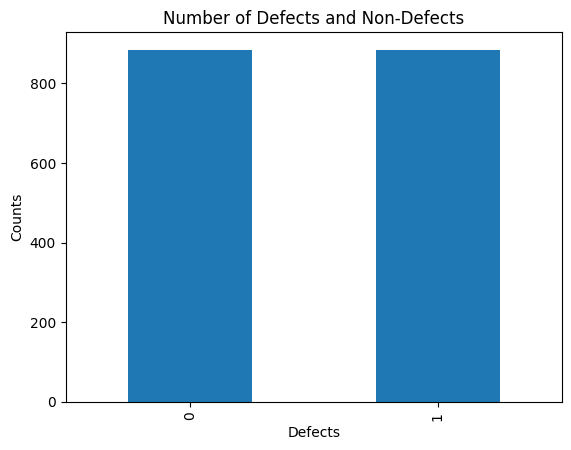
\includegraphics[width=0.7\textwidth]{./figures/balanced_data.png}
    \caption{Data distribution after using SMOTE}
    \label{fig:smote_plot}
\end{figure}

\subsection*{Results}
We trained SVM, Random Forest, Logistic Regression, and Ensemble models on the
balanced dataset and evaluated their performance. The results showed a
significant improvement in the performance of all models, particularly in the
classification of the minority class (1). The best performance was observed
with the Random Forest model, which achieved a precision of 0.92, recall of
0.96, and f1-score of 0.94 for the minority class (1).

\begin{table}[ht]
    \centering
    \begin{tabular}{|c|c|c|c|c|}
        \hline
        Model                     & Class   & Precision & Recall & F1-score \\
        \hline
        SVM                       & Class 0 & 0.93      & 0.99   & 0.96     \\
        SVM                       & Class 1 & 0.00      & 0.00   & 0.00     \\
        \hline
        Random Forest             & Class 0 & 0.93      & 0.98   & 0.95     \\
        Random Forest             & Class 1 & 0.20      & 0.07   & 0.11     \\
        \hline
        Logistic Regression       & Class 0 & 0.92      & 0.97   & 0.95     \\
        Logistic Regression       & Class 1 & 0.00      & 0.00   & 0.00     \\
        \hline
        Ensemble Model            & Class 0 & 0.93      & 0.98   & 0.95     \\
        Ensemble Model            & Class 1 & 0.00      & 0.00   & 0.00     \\
        \hline
        SVM SMOTE                 & Class 0 & 0.84      & 0.83   & 0.83     \\
        SVM SMOTE                 & Class 1 & 0.82      & 0.83   & 0.82     \\
        \hline
        Random Forest SMOTE       & Class 0 & 0.96      & 0.92   & 0.94     \\
        Random Forest SMOTE       & Class 1 & 0.92      & 0.96   & 0.94     \\
        \hline
        Logistic Regression SMOTE & Class 0 & 0.77      & 0.85   & 0.81     \\
        Logistic Regression SMOTE & Class 1 & 0.82      & 0.73   & 0.77     \\
        \hline
        Ensemble Model SMOTE      & Class 0 & 0.85      & 0.87   & 0.86     \\
        Ensemble Model SMOTE      & Class 1 & 0.86      & 0.83   & 0.85     \\
        \hline
    \end{tabular}
    \caption{PC1 Dataset Model Performance Analysis on Balanced Data.}
    \label{tab:PC1 Performance Analysis Balanced Data}
\end{table}
\newpage
\bibliographystyle{plain}
\bibliography{references}
\end{document}
